%
% File: chap01.tex
% Author: Hongliang Zhong
% Description: Introduction chapter where the biology goes.
%
\let\textcircled=\pgftextcircled
\chapter{Introduction}
\label{chap:introduction}
\begin{quote}
``Bandit problems embody in essential form a conflict evident in all human action: choosing actions which yield immediate reward vs. choosing actions whose benefit will come only later.''
\hfill
-- P.~Whittle (1980)
\end{quote}
\begin{figure}[h!]\centering{

\includegraphics[width=0.33\linewidth]{chapters/chapter01/fig01/bandit.png}
\hspace{-0.75cm}

\includegraphics[width=0.33\linewidth]{chapters/chapter01/fig01/bandit.png}
\hspace{-0.75cm}

\includegraphics[width=0.33\linewidth]{chapters/chapter01/fig01/bandit.png}
}
\end{figure}

\initial{E}arly in 1933, William R. Thompson described a method ``Thompson Sampling'' in article \cite{thompson1933likelihood}, for attempting to compare treatments which both have unknown effectiveness. Here, it is a focus on finding the balance between exploration and exploitation. This is the prototype of bandit problems. 

In 1952, H. Robbins introduced a problem in \cite{robbins1952bandit}, which worked in the area of sequential selection of experiments, and became the foundation of Bandit problem. 

In 1957, Richard Bellman wrote the first book\cite{bellman1957markovian} at this subject, formulated the Multi-Armed Bandit problem as a class of dynamic program. 


Related to H. Robbins's research, in 1979, Gittins and Jones published \cite{gittins1979dynamic} to outline an allocation index for sequential experiment problems, and defined the stopping rule by the theorem. From then on, more and more proofs of ``Gittins Index'' have been proposed, i.e. by Whittle \cite{whittle1980multi},  Weber \cite{weber1992gittins}, Tsitikis \cite{tsitsiklis1994short}, $\dots$

Nowadays, Further researches and applications of Bandit problem have been explored,  for example, in Machine Learning by  \cite{Berry85Bandit, kaelbling1996reinforcement,Sutton98}, Economics \cite{anderson2001behavioral,banks1997experimental,steyvers2009bayesian} , Cognitive Science  \cite{daw2006cortical}, etc.
%The classical Bandit modeling, named ``K-Armed Bandit'', that the gambling machines has $K$ arms, for each arm with an unknown, possibly different distribution of payoffs. You have no idea which arm has the most reward. After some times experiments, you can earn some knowledge of them ( it could be the reward of each arm by observing temporal of each time). Therefore, you should trade off a balance between to gain the most rewards and to gain the new knowledge, that's the core philosophy thought of Bandit problem. For example, always pull the arm who performed best in past, maybe you miss the optimal arm by a local optimal arm. For more details of trade-off between Exploration/Exploitation, we will introduce it in the Chapter~\ref{chap:tradeoff}.

\
\
\
\
\
\


%=======

\section{Modeling of Bandit Problems}
\label{sec:modeling}

Consider the Robbins's sequential decision experiment\cite{robbins1952bandit}, there are several possible choices (finite arms or infinite arms). Generally, we should make a choice from the set of arms at each time. After observation, you will receive a boolean feedback $\mathbf{1}$ or $\mathbf{0}$  as reward. 
Whatever the feedback is, it is always the useful knowledge to make prediction in future from the past. We can even estimate the fixed but unknown distribution of arms by the reward of each time. The goal of bandit problems, is to maximize the received rewards from all steps, minimize the cumulative regret and find the optimal arm (the set of optimal arms). 

The bandit problem can be defined by the number of trials, as the ``finite horizon'' or ``infinite horizon''. The former has a number of trials fixed and small, the latter's trials number usually unknown in advance, but has some probability at any trial will be the last; by the number of arms, it could be divided into ``two arms'', ``K-armed'' and ``Many-armed'' Bandits; by the environment, it is divided into ``Stationary bandit'', ``Non-stationary bandit'', ``Adversary bandit'' and ``Contextual bandit''.

In the next chapters, we will tell about each kind bandits, their performance, properties and caracteristics. Specially, we will emphasize on Chapter~\ref{chap:BF} and Chapter~\ref{chap:momab}, to propose the novel solutions and algorithms. Here, we address a simple process in order to introduce the core thought of Bandit problems. Just like we have introduced , the target of bandit problems is to maximize the number of rewards over all steps. Generally, in the first few trials, pursuing the goal might involve trying different arms, getting some knowledge of which arms may be rewarding or which may not. Towards to the end, it will become increasingly important to pull the same  arm repeatedly by the same reasonable strategy. Where the way to check out some uncertain arms is called ``Exploration'', and the ways to choose the arm (a set of arms) that is more certain by the reasonable strategy is called ``Exploitation''. 
The decisions are always depending on the potential knowledge of the optimal arms in the setting. If the setting is believed to have optimal arms, then others will be encouraged to try of arms. On the other hand, if the setting has a bad reputation for arm quality, a modest reward rate encourages repeat choice.

Performing well on bandit problems, requires to keep a balance between Exploration and Exploitation during decisions. In early steps, it makes sense to explore, to search for those with the highest reward rates. In later times, it makes sense to exploit those arms known to be good, maximizing the reward for each current decision. How to keep balance between Exploration and Exploitation, ( the details shown in the Chapter~\ref{chap:MAB} ), it should be influenced by factors such as the distribution of reward rates, the total number of plays, etc.

We also attempt to construct the bandit models that capture individual differences and collective performance in solving bandit problems. Differences in how people solve the bandit problems that involve optimization and classification under interactive constraints, provide a window onto variance in cognitive abilities. Recently, take attention to some mechanism, a process of taking into account the collective ability of a group of individuals to solve a task, has discovered that a large group's aggregated answers to questions involving quantity estimation and general world knowledge are as good as, and often better than, the answer given by any of the individuals within the group (e.g.\cite{surowiecki2005wisdom}). We are thus interested in whether this phenomenon also applies to sequential tasks such as bandit problems whether a collective decision-making through aggregating methods can achieve better outcomes than most of the individuals.

From the theorem view, we also care about how to find optimal solutions for bandit problems that make model evaluation and model comparisons more efficient. We dedicate next chapters of this dissertation to our effort on this problem.

\section{Applications of Bandit Problems}
\label{sec:application}
The development of Bandit Problems is rapid, mainly due to its applications and prospects are very impressive.

Early in 1933, Dr. Thompson encountered a difficulty: to treat a same disease, there may be two or even more solutions, but their effectiveness are unknown. Actually, it is also the problem that Bandit problems need to solve, find the best choice on facing some  unknown probability distributions. At that time, Thompson proposed the ``Thompson Sampling''(details in Chapter~\ref{chap:MAB}), a prototype of Bandit problem.
\begin{figure}[!h]
\centering{
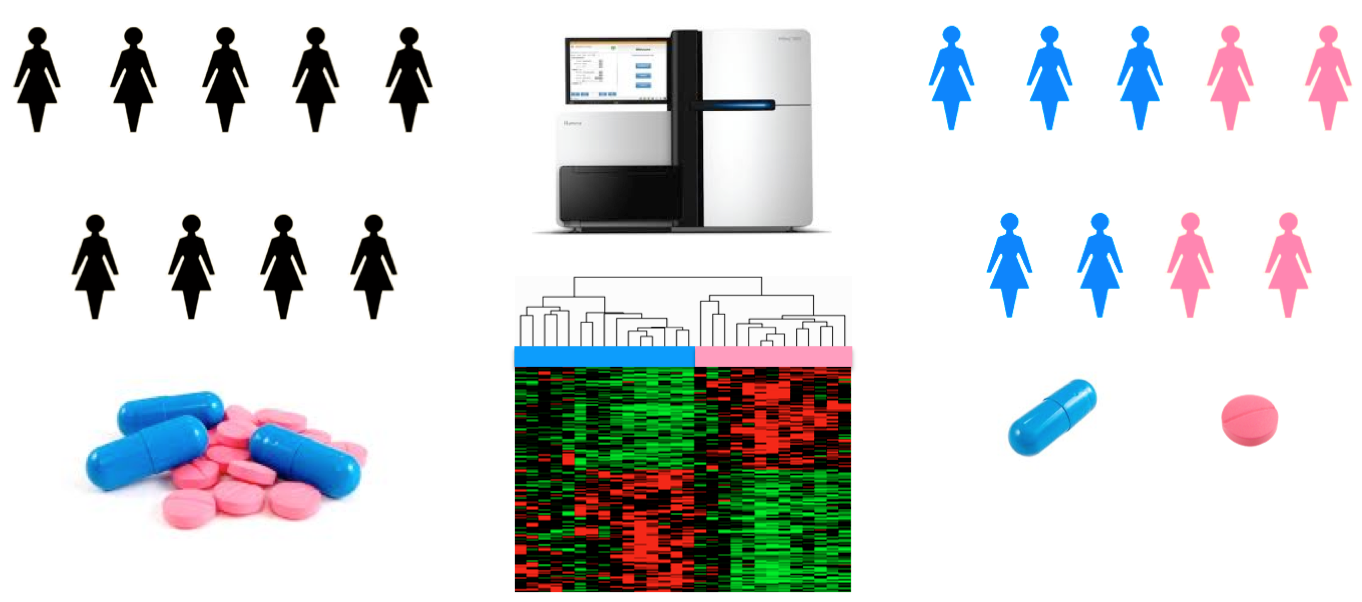
\includegraphics[width=0.6\linewidth]{chapters/chapter01/fig01/clinicaltrials.png}}
\caption{Clinical Trials}
\end{figure}

Nowadays, with the rising development of Internet, the Bandit problems become extremely popular. Such as personalized search, Internet advertising etc. For these applications, Operators will give each user a certain number of recommendations. sometimes, there are some user-friendly, but sometimes not. For traditional way, the supervised learning should get full feedback from users, if there is no interested recommendation. But most users do not like give this full feedback. In this case, Bandit feedback is proposed.(Details will be shown in Chap~\ref{chap:MAB})
\begin{figure}[!h]
%\label{fig:websearch}
\centering{
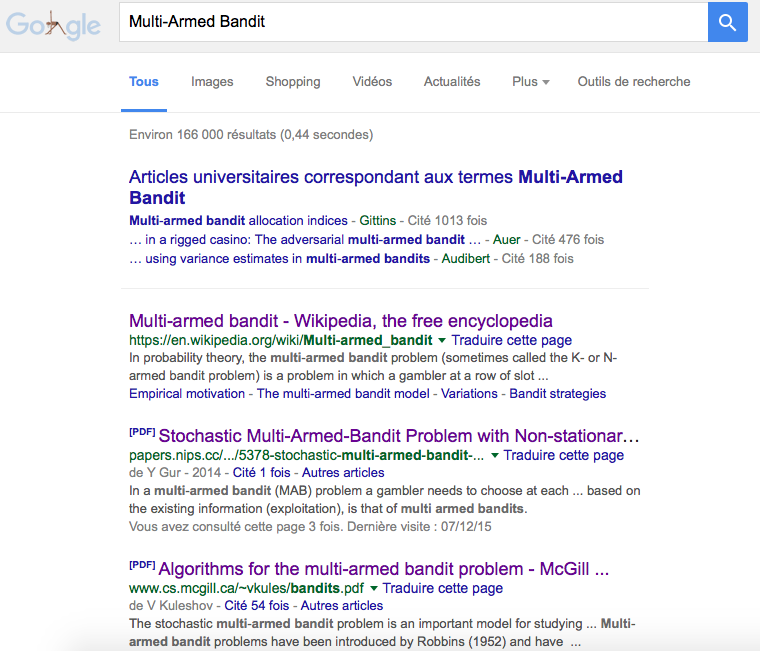
\includegraphics[width=0.6\linewidth]{chapters/chapter01/fig01/websearch.png}
\caption{Web Search}}
\end{figure}

Otherwise, Google proposed an analytic service based on the method of Multi-Armed Bandit(Chapter~\ref{chap:MAB}). It is an analytic system to compare and manage some online experiments. For each experimentation, maybe there are a variety of alternative solutions. In past, it is usually used A/B test to solve, but A/B test cost much and waste time. So google takes Bayes Theorem combining Multi-Armed Bandit, it could reduce much time and get higher accuracy than ever.
\begin{figure}[!h]
\centering{

\includegraphics[width=0.6\linewidth]{chapters/chapter01/fig01/googleanalytic.png}
}
\caption{Google Analytic}
\end{figure}

Except Internet, Bandit problems also have very broad prospects in other domains. Such as in World War II, many countries had tried to solve multi-objective multi-tasking attack, this one could be considered as Multi-Objective Multi-Armed Bandit problem (shown in Chapter~\ref{chap:momab}). Otherwise, queueing and scheduling(\cite{veatch1996scheduling,ehsan2004optimality}), stock in non-stationary(\cite{garivier2008upper}) etc, all of them will be the direction to be committed to develop for Bandit problems.

\section{The structure of thesis}
\label{sec:structure}

This dissertation consists of 5 Chapters followed the discussion of Bandits Problem. This first Chapter, proposed the background of Bandit problems.

Chapter 2, is about some important strategies of Bandit problem, how to trade off the balance between Exploration/Exploitation. In this chapter, we introduce some methods very useful and effective to keep balance for the tradeoff. Furthermore, to analyze their advantage and disadvantage with principal theorem and empirical experiments. The classical Bandit problem, Multi-Armed Bandit problem, will be introduced. Recently, there are many researches working in this setting. We concentrate on its environment, lower bound, gittins index and best arm identification etc.

Chapter 3, it's the classification problem under Bandit Feedback. Here, we proposed several algorithms in the-state-of-art to solve the problems in multiclass or multilabel classification. Compared those algorithms, we will introduce the algorithms who related or modified from those classification algorithms. At last, compare their effectiveness or regret bound by empirical experiments based on those common data sets.

Chapter 4, it is the extension of Multi-Armed Bandit that each arm has multi-objective. So many domains are met this problem, i.e. supply chain, some decision system, Big data platform and so on. In this chapter, we will introduce some traditional way to solve this problem, and our contribution, a novel method who works more effectively and more precisely.

Chapter 5, also the last chapter. We will make the conclusion of all chapters in this part.

%=========================================================